\documentclass[../Cours.tex]{subfiles}

\begin{document}
\chapitre{Angles}

\partie{Concept}

\definition{Un angle représente l'écartement entre deux demi-droites partageant la même origine.}

\illustration{%
\begin{center}
\begin{tikzpicture}
    \coordinate (O) at (0,0);
    \coordinate (A) at (2,0.5);
    \coordinate (B) at (2,-0.5);
    \draw ($(O)!1.5!(A)$) -- (O) -- ($(O)!1.5!(B)$);
    \draw[rouge,fill=rouge] ($(O)!0.5cm!(A)$) arc (15:-15:0.5) -- (O) -- cycle;
    \node at (A) {|};
    \node[above left] at (A) {$A$};
    \node at (B) {|};
    \node[below left] at (B) {$B$};
    \node[left] at (O) {$O$};
    \node[anchor=west] at (2.5,0) {\textcolor{rouge}{L'angle $\widehat{AOB}$}};
\end{tikzpicture}
\end{center}
}

\definition{%
\begin{itemize}
    \item Le \emph{sommet} de l'angle est l'origine commune.
    \item Les \emph{côtés} de l'angle sont les demi-droites.
\end{itemize}
}

\notation{Trois points avec un << chapeau >> \\ Le point du milieu est le sommet}

\partie{Les types d'angles}

\souspartie{Les angles saillants et rentrants}

\definition{%
\begin{itemize}
    \item Un angle saillant est un angle dont la mesure est comprise entre \ang{0} et \ang{180}.
    \item Un angle rentrant mesure entre \ang{180} et \ang{360}.
\end{itemize}
}

\illustration{%
\begin{center}
    \begin{tikzpicture}
        \coordinate (E) at (0,0);
        \coordinate (D) at (2,0.5);
        \coordinate (F) at (2,-0.5);
        \draw ($(E)!1.5!(D)$) -- (E) -- ($(E)!1.5!(F)$);
        \draw ($(D)+(0,0.1)$) -- ($(D)+(0,-0.1)$);
        \draw ($(F)+(0,0.1)$) -- ($(F)+(0,-0.1)$);
        \node[above right] at (D) {$D$};
        \node[below right] at (F) {$F$};
        \node[left] at (E) {$E$};
    \end{tikzpicture}
\end{center}
}

\propriete{La somme d'un angle saillant et de l'angle rentrant qui lui est associé vaut \ang{360}.}

\exemple{$\widehat{DEF} + {DEF} = \ang{360}$}

\souspartie{Nomenclature des angles saillants}

\renewcommand*{\arraystretch}{3}
\begin{tabularx}{\textwidth}{|l|C|X|}\hline
    aigu & entre \ang{0} et \ang{90} & \makecell{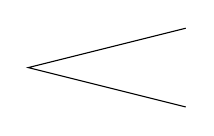
\begin{tikzpicture}
        \coordinate (E) at (0,0);
        \coordinate (D) at (2,0.5);
        \coordinate (F) at (2,-0.5);
        \draw (D) -- (E) -- (F);
    \end{tikzpicture}}  \\\hline
    droit & $= \ang{90}$ & \makecell{\begin{tikzpicture}
        \coordinate (E) at (0,0);
        \coordinate (D) at (2,0);
        \coordinate (F) at (0,1);
        \draw (D) -- (E) -- (F);
    \end{tikzpicture}} \\\hline
    obtus & entre \ang{90} et \ang{180} & \makecell{\begin{tikzpicture}
        \coordinate (E) at (0,0);
        \coordinate (D) at (2,0);
        \coordinate (F) at (-1,1);
        \draw (D) -- (E) -- (F);
    \end{tikzpicture}} \\\hline
    plat & $= \ang{180}$ & \makecell{\begin{tikzpicture}
        \coordinate (E) at (0,0);
        \coordinate (D) at (2,0);
        \coordinate (F) at (-2,0);
        \draw (D) -- (E) -- (F);
    \end{tikzpicture}} \\\hline
\end{tabularx}
\renewcommand*{\arraystretch}{1}

\end{document}